\graphicspath{{figures/intro/}}
\chapter{Analysis}\label{ch:analysis}



\section{Behavioural Analysis of Zebrafish}
Zebrafish are very social animals and have tendencies to form groups \citep{RahmanKhan2018}. An aggregation of zebrafish can be either a shoal or a school depending on whether the zebrafish are interacting socially or not. When an aggregation of zebrafish is due to social interaction, the zebrafish are shoaling and the swimming pattern is chaotic, but when zebrafish are schooling, the swimming pattern is tightly coordinated and organised \citep{Miller2012a}. Identification of the swimming pattern can thereby be studied to investigate social phenotypes and behavioural patterns when affected by a certain drug or pheromone \citep{RahmanKhan2018}. 

\cite{Kalueff2013} describes multiple scenarios in which the zebrafish is prone to sudden changes in both speed and direction. Depending on the situation, the zebrafish can move very erratic often reflecting a state of anxiety or fear. Furthermore, sudden bursts can also occur in an attempt to attack another fish, often connected to social dominance \citep{Kalueff2013}.

As mentioned, the zebrafish is also used to test the general behaviour when affected by a drug. This is done by having a control group of zebrafish and recording the normal behaviour in an aquarium and then comparing this behaviour with a drug affected behaviour \citep{Stewart2015}. \autoref{fig:drug_effect} shows an example of swimming patterns of zebrafish under influence of different drugs made by \cite{Stewart2015}. It is clear how the drugs changes the swimming patterns of a zebrafish, which may be transferable to how it will affect humans as well.\\ 

\begin{figure}[h]
	\centering
	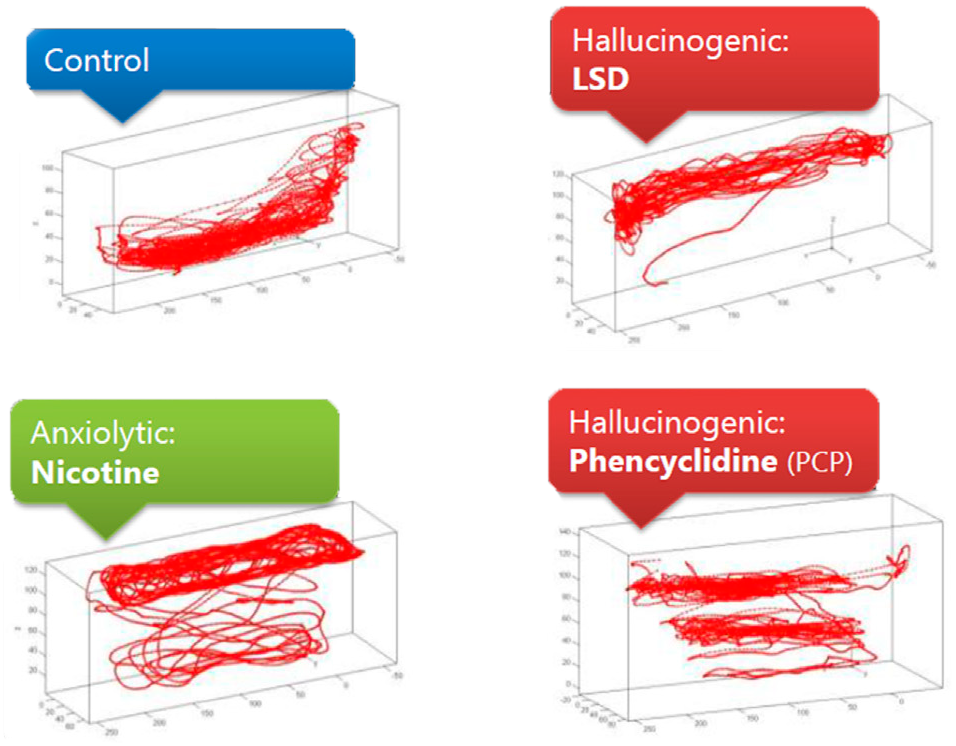
\includegraphics[width=0.8\textwidth]{drug_effect}
	\caption{Zebrafish swimming behaviour under influence of drugs, by \cite{Stewart2015}}
	\label{fig:drug_effect}
\end{figure}


\section{Tracking of Zebrafish}

To investigate the difference in behavioural patterns, i.e. due to drugs, each zebrafish must be detected individually over time. Detection of the zebrafish is often done with an automated tracking system, as done by \cite{Stewart2015}, as manual annotation of the data often proves infeasible.

\subsection{Tracking Requirements}
In order to be able to track zebrafish, collection of data is firstly necessary. Recording of the zebrafish is done using one or more cameras either from the top of the aquarium or looking into the aquarium from the side.

Due to the erratic movement of the zebrafish, the higher the \gls{fps} the camera is able to capture video at, the better, as this will increase the probability of the camera capturing every movement of the fish. \cite{Pedersen2017} states, that even at 240 \gls{fps} the zebrafish is still somewhat blurred when accelerating, which can lead to a lower detection rate.

The top down view of the aquarium when recording, is often used when using a single camera setup. The top view takes advantage of the uniform and rigid head physiology of the zebrafish. Even though the zebrafish is able to contort its body, the head most often remains the same, when using the top view. Examples of the rigid head is shown in \autoref{fig:rigid_head}.

\begin{figure}[H]
	\centering
	\begin{subfigure}[b]{0.3\textwidth}
		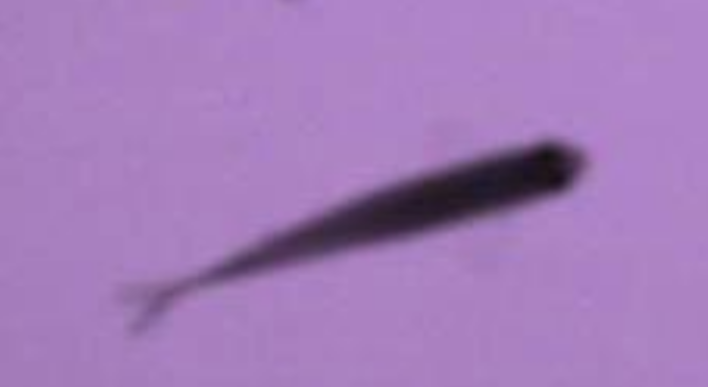
\includegraphics[width=\textwidth]{head_straight}
		\label{fig:head_straight}
	\end{subfigure}
	\begin{subfigure}[b]{0.3\textwidth}
		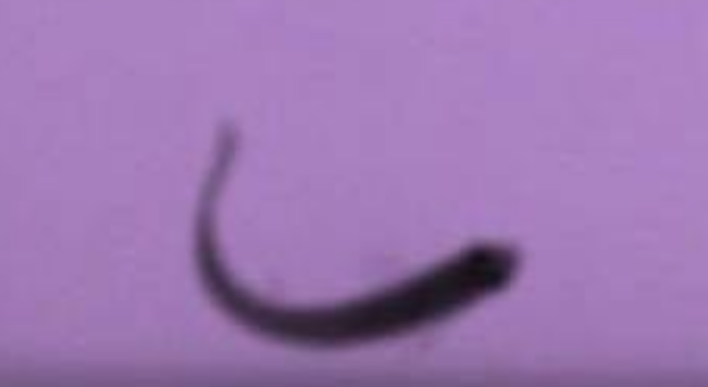
\includegraphics[width=\textwidth]{head_bend}
		\label{fig:head_bend}
	\end{subfigure}
	\begin{subfigure}[b]{0.3\textwidth}
		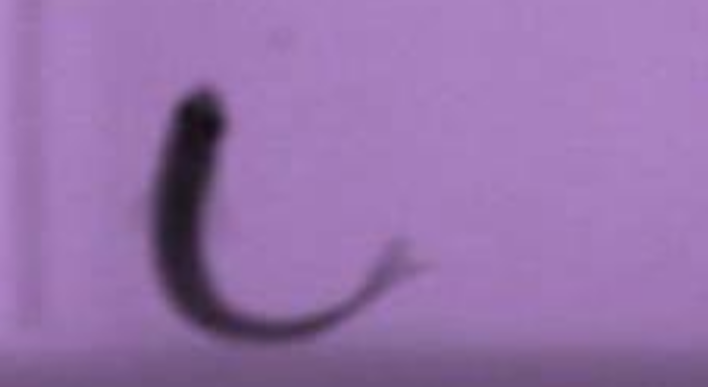
\includegraphics[width=\textwidth]{head_bend2}
		\label{fig:head_bend2}
	\end{subfigure}
	\caption{Examples of the rigid head of the zebrafish in different grades og contortions of the body}
	\label{fig:rigid_head}
\end{figure}

The data shown in \autoref{fig:rigid_head}, is captured from above the aquarium with a \gls{nir} backlight beneath the aquarium.\\

When recording from the side of the aquarium more details of the fish is available, as the zebrafish has uniquely coloured stripes on both sides, which can be used to identify the zebrafish \citep{Karpova2018}.

According to \cite{Qian2017}, due to the shape of the zebrafish, it generally takes up more space when filmed from the side than from a top view. Furthermore, when the zebrafish turns towards or away from the camera, the shape will be very different than when looking at the side of the zebrafish \citep{Pedersen2017}. Examples of both a regular side view and some issues from the view is shown in \autoref{fig:side_view}.

\begin{figure}[H]
	\centering
	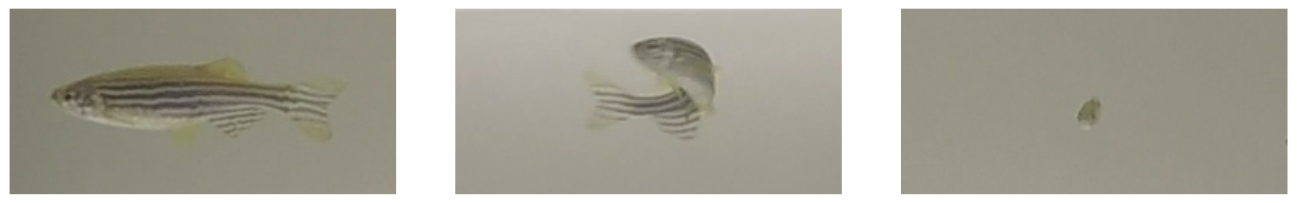
\includegraphics[width=0.9\textwidth]{side_view}
	\caption{Examples of positions of zebrafish in the side view. Image from \cite{Pedersen2017}}
	\label{fig:side_view}
\end{figure}

When data is acquired, it will need to be prepared before tracking or annotating is done. 

\subsection{Annotating Data}

Annotating data is understood as manually marking each zebrafish/object in every frame of a video, whereas, when using an automated solution it can also be referred to as tracking system. 

A tracking system can be split into multiple steps:

\begin{itemize}
	\item Pre processing
	\item Detection
	\item Create trajectories
\end{itemize}

\subsubsection{Pre Processing}
When making operations on a video, the file is split into individual frames, and every frame is treated as an individual image. Before locating of the zebrafish in the image is done, some pre processing of the image is often performed. This often includes removing the background and noise from the image.

This is done to ease the process of locating the zebrafish as it will be isolated in the image.

\subsubsection{Detection}
Detection of the zebrafish is done in multiple ways. A detection will ultimately produce a single point in the image.

Head detection of the zebrafish is an often used approach due to the rigid head of the zebrafish. This means the head will keep the same shape while swimming, whereas the rest of the body may change shape, which will make it harder to detect if focus is on the entire zebrafish.

Other examples of detection, are centre of mass of the zebrafish or extracting a skeleton of the zebrafish, representing the shape of the object with a line. Finding the centre of mass of the zebrafish, if not being limited, may end up outside of the object if it is bending into a shape looking like a C.

Examples of extracted points from detections are shown in \autoref{fig:det_point}.

\begin{figure}[H]
	\centering
	
\includegraphics[width=\textwidth]{det_point}
	\caption{Examples of extracted points from detections. The first fish is head detection, the second is centre of mass, and the third is skeletonisation}
	\label{fig:det_point}
\end{figure}

\subsubsection{Create Trajectories}
When the desired point in the zebrafish is extracted, the point needs to be linked together to create a trajectory. If only a single zebrafish is present in the aquarium no identification is necessary, as every point found belongs to one individual.

As soon as multiple fish are present in the aquarium at the same time, a decision needs to be made to connect the previous frame's detections to the new ones in the current frame. This can be done by predicting where each individual will be in the following frame based on a state vector and experience from previous frames as input to a Kalman filter, which then makes a qualified guess based on statistics of the new positions. Besides a Kalman filter, a simple cost function such as the Hungarian algorithm can be applied to link detections.\\

An issue occurring when multiple zebrafish are in the same aquarium, is when two or more individuals lie close enough together or on top of each other, which may confuse or trick the prediction and cost algorithm.

\subsection{Occlusions}
An occlusion is when one object is hidden or overlapped by another object from a specific point of view e.g. from the camera view. When a zebrafish occlude another there is a risk of losing the detection and thereby the position of the occluded fish in one or more concurrent frames. According to  \cite{Green2012} the use of automated tracking systems perform with same accuracy as manual annotations but in a faster manner. However, they state that automated tracking systems have complications with occlusions. 

When a detection is lost due to an occlusion, the identity of the zebrafish may be lost as well. If no re-identification is employed in a tracking system, a new ID may be assigned to the object which was lost due to an occlusion. This scenario is visualised in \autoref{fig:re-id_Ex}

\begin{figure}[H]
	\centering
	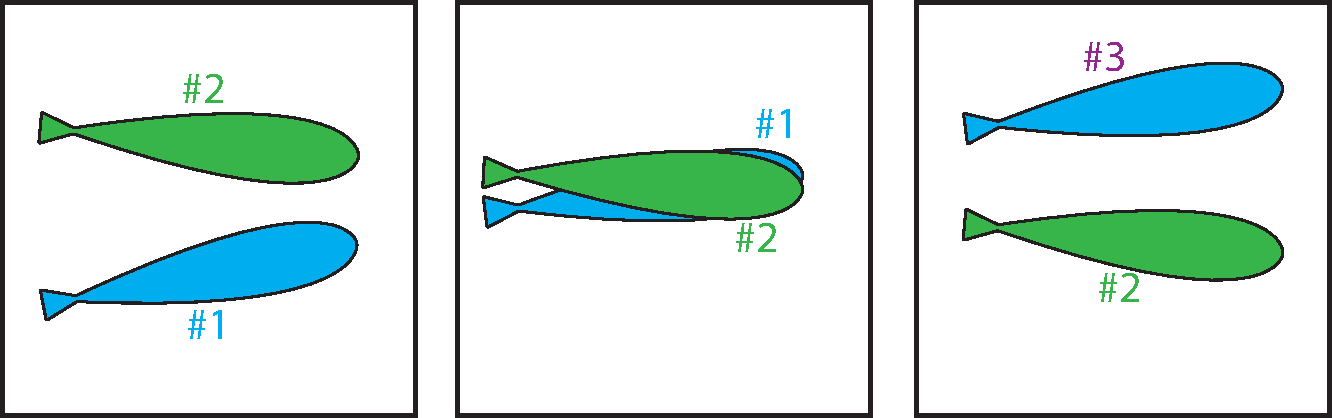
\includegraphics[width=0.9\textwidth]{re_id_ex}
	\caption{Re-ID scenario due to occlusion}
	\label{fig:re-id_Ex}
\end{figure}

Not all occlusions will cause the same types of complications, and some occlusions do not cause any disruption of the trajectory. This is determined by the detection system deployed to track the zebrafish. If the detection of a zebrafish is centred at the head, no occlusion will be detected when only the bodies of two zebrafish overlap, however, if detection is done by either skeletonisation or centre of mass, an occlusion will most likely occur \citep{Feijo2018}. An example of this scenario is shown in \autoref{fig:system_dep_occl}.

\begin{figure}[H]
	\centering
	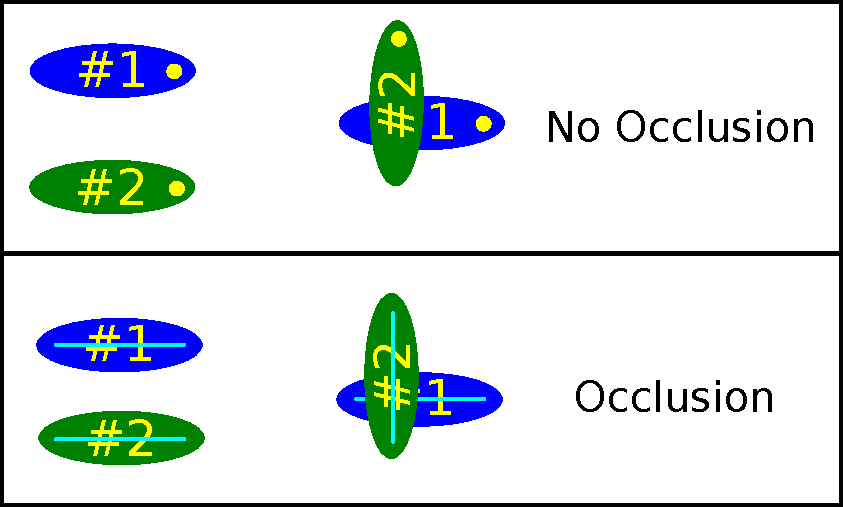
\includegraphics[width=0.85\textwidth]{system_dep_occl}
	\caption{Different types of detection leads to different types of occlusion}
	\label{fig:system_dep_occl}
\end{figure}

Missing detections and wrong identifications are undesirable, as this will require a user of the tracking system to intervene and correct the errors, which will prolong the process. Therefore, solutions to either handling the occlusions or automatically solving the wrong identification are often implemented in a tracking solution.

\subsection{Object Detection}\label{sec:obj_det}
In order to be able to detect the zebrafish occlusions in every frame, object detection is necessary. Object detection is defined as an employment of computer vision which recognises unique features of objects in an image.

Object detection consists of two main tasks; classification and localisation. It can furthermore be split into two categories depending on the amount of classes which must be detected. If it is only one class, such as detecting humans in an image or detecting any kind of zebrafish occlusion, it is known as class-specific detection. Whereas detecting multiple different kinds of objects is knows as multi-class detection  \citep{Zhang2013}.

The main objective of an object detector is to generate a label list of predefined objects detected in an image. The list should specify which classes are present and where in the image they are located.\\

\subsubsection{Deep Learning}
When using deep learning and a \gls{cnn} for object detection one of the earliest implementations was the \gls{rcnn}. As the name suggests, the method is based upon a region proposal based \gls{cnn} instead of using the often previously used sliding window technique which some times can lead to a large amount of testing windows.

The \gls{cnn} used in the \gls{rcnn} is utilised for feature extraction feeding into a class-specific \gls{svm} to categorise each object. The \gls{cnn} is pre-trained on the ImageNet database and then trained on the PASCAL VOC dataset. An overview of the \gls{rcnn} pipeline is shown in \autoref{fig:rcnn_pipe}. More in-depth of deep learning is found in \autoref{ch:design}.

\begin{figure}[h]
	\centering
	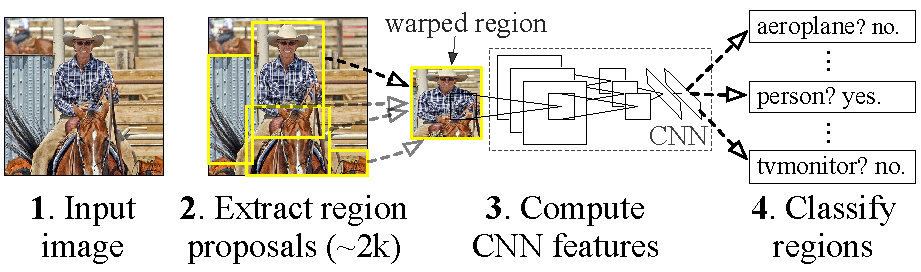
\includegraphics[width=0.9\textwidth]{rcnn_flow}
	\caption{Simple flow diagram of the R-\gls{cnn} by \cite{Girshick2014}}
	\label{fig:rcnn_pipe}
\end{figure}

As shown in \autoref{fig:rcnn_pipe} the \gls{rcnn} is split into 3 individual steps consisting of; region proposals, feature extraction, and \gls{svm} classification.\\

The region proposals are extracted using \textit{SelectiveSearch} which initialises regions in the image and then merge these with a hierarchical grouping \citep{Uijlings2013}. The final grouping is then a box containing the entire image. The regions are grouped in relation to colour space and similarity \citep{Girshick2014}. 

The next step in the solution is warping the proposed regions to fit the \gls{cnn} input size and extracting features from these and produce a $4096$ dimensional feature vector. The feature vectors consist of both positive and negative proposals found with the SelectiveSearch. These vectors are used to train the class specific \gls{svm}s, one \gls{svm} per class in which a background class is included \citep{Girshick2014}.
When testing a given image, the SelectiveSearch generates approximately 2000 proposals, which each are propagated through the \gls{cnn} to extract feature vectors. Each feature vector is tested against every class-specific \gls{svm}. To remove overlapping detections a greedy Non-maximum Suppression is applied \citep{Girshick2014}.

At the time of publication, the \gls{rcnn} achieves state of the art performance in object detection, with a $~13\%$ increase in precision compared to the previously best method \citep{Girshick2014}.

The \gls{rcnn} does leave room for improvements as it is a slow solution when testing on an image. Furthermore, as the solution is split into multiple modules, the loss calculations for training the \gls{svm}s is not used to update the \gls{cnn}.\\

An improvement on both speed and accuracy of the \gls{rcnn} was published a year later, called Fast \gls{rcnn}. Instead of using the multi module pipeline, as illustrated in \autoref{fig:rcnn_pipe}, training is now done end-to-end. The solution takes an image  and a set of pre-computed object proposals, like the \gls{rcnn} \citep{Girshick2015}.

Instead of individual proposals as in the original \gls{rcnn}, the new iteration propagates the entire image forward through multiple convolutional and max-pooling layers to produce a feature map. The features are extracted from each proposal using a \gls{roi} pooling layer. After the \gls{roi} pooling layer follows two fully connected layers leading to two different outputs; a softmax classification layer and a bounding box regression layer \citep{Girshick2015}. This pipeline is also shown in \autoref{fig:frcnn_pipe}.

\begin{figure}[H]
	\centering
	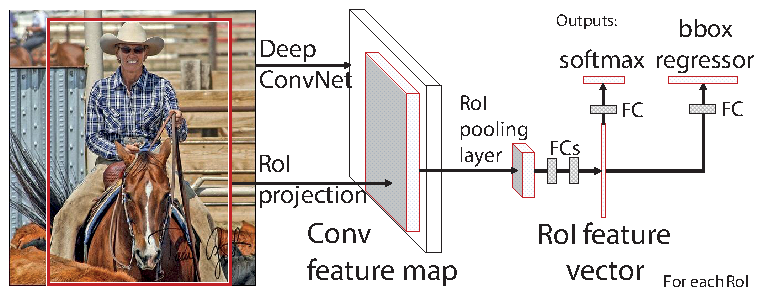
\includegraphics[width=0.9\textwidth]{frcnn_pipe}
	\caption{Fast \gls{rcnn} pipeline overview, by \cite{Girshick2015}}
	\label{fig:frcnn_pipe}
\end{figure}

Just like the \gls{rcnn}, the Fast \gls{rcnn} is pre-trained using the ImageNet database fine tuned for object detection, but instead of being based on AlexNet, as \gls{rcnn} is, the best performing solution of Fast \gls{rcnn} is based on the deeper VGG16 network \citep{Girshick2015}. When comparing to the previous iteration, \gls{rcnn}, it is done while both solutions are using the VGG16 network layout instead of the AlexNet for the \gls{rcnn}. This is done to have a common ground for comparison. Fast \gls{rcnn} improves precision with $4\%$ \citep{Girshick2015}.

The main improvement of the new model is more in speed both in training and testing due to the computing of a convolutional feature map for the entire image. The speed increase is only in relation to the actual detection, as the regions proposals are slow and create a bottleneck for the system \citep{Girshick2015}.\\

To combat the slow region proposals of Fast \gls{rcnn}, \cite{Ren2017} created a third iteration of the \gls{rcnn} network called \textit{Faster \gls{rcnn}}. Here a network named Region Proposal Network (RPN) is implemented to compute region proposals as part of a  network. The RPN shares the convolutional layers and the feature map with the \gls{roi} pooling in the Fast \gls{rcnn}. Due to the layers being computed on the entire image, the time used for proposals generated using the RPN is much lower than of a method such as SelectiveSearch. The RPN, computing region proposals, is the only new part of the Faster \gls{rcnn} compared to Fast \gls{rcnn}.

The results of the Faster \gls{rcnn} in precision are rather small, but the entire computing time of the solution has been significantly minimised, from about $2$ seconds per image to $0.2$ seconds, including region proposals for both timings.

Multiple solutions on the \gls{coco} dataset object detection leader board are still employing the framework of \gls{rcnn} and its predecessors, which shows why the \gls{rcnn} is still a state of the are solution.


\subsection{Handling Occlusions}
According to a study by \cite{Qian2017}, occlusions will occur both while recording from above and from the side of an aquarium, but with greater occurrence from the side of the aquarium due to the shape of the zebrafish. As previously mentioned, occlusions can cause errors, resulting in missing data for an individual due to a new ID \citep{Feijo2018}.\\

A solution to missing tracking data due to occlusions, is to re-link parts of the trajectories (tracklets) to create complete trajectories. This can be done by computing a state vector for each zebrafish and using a Kalman filter which makes predictions of the fish’s position, and thereby estimate what ID belongs to the different zebrafish after an occlusion \citep{Feijo2018, Qian2014}.

To avoid patching in missing data, another more feasible solution could be made to solve occlusions before they occur by detecting the zebrafish in each frame. Both \cite{Romero-Ferrero2019} and \cite{Dolado2014} propose solutions which detect occlusions in an effort to solve them using computer vision. \cite{Dolado2014} has categorised occlusion types by how the zebrafish overlap each other in an effort to specify the solution. However, the only way they solve the occlusions are through a two-step trial and error process i.e. if the first step does not solve the solution, the second step is applied, without factoring in the occlusion type. 
However, a novel approach could be to recognise an occlusion type in order to apply a predefined optimal solution.


\section{System Dependencies}\label{sec:int_dep}
Different types of tracking systems may vary in requirement of user interaction throughout the tracking. The ability of the solution may require the user to interact with the system when occlusions occur in the video data in order to pick the correct path for each zebrafish and thereby solve or fix the data. 

If a solution has a high level of user interaction, localisation of an occlusion may not be a requirement due to the necessary interactions of a user, but recognition of an occlusion occurring in the image may be sufficient.\\

With this analysis a specification of the problem sought out to solve is presented in the following chapter.
%An object tracking solutions consists of multiple steps towards creating complete trajectories for each object in an arena. As stated in \autoref{ch:related}, occlusions often lead to issues in tracking solutions and are often not handled to completion. This leads to missing data which a user must handle either by annotating some of the data themselves or using the data incomplete.
%
%To combat this, some solutions choose to solve the occlusions \citep{Romero-Ferrero2019, Dolado2015}. By being able to detect when an occlusion occurs a process of handling them is initiated.
%
%Both \cite{Romero-Ferrero2019} and \cite{Dolado2015} initially counts the amount of objects in the each frame and compare it to the given amount of object which are supposed to be in the frame.\\
%
%An implementation of an occlusion detection solution can be categorised as a single step in an object tracking system. The detection step would consist of detecting occlusions in every frame, categorising the type of occlusion and extracting the occlusion position in the image. This is also show in an flowchart overview in \autoref{fig:overview_flow}.
%%Problem analyse. Hvad er det jeg/vi vil løse og hvorfor? Skal lægge op til problem formuleringen.
%
%Often, before any kind of detections take place some pre processing of the image is done \citep{Delcourt2018}. This would be any kind of alternations made to the image, which will make it easier to isolate the desired objects from the rest of the image.
%
%An implementation of an occlusion detection solution must be placed before the tracking of the objects in a object tracking pipeline, as the handling of occlusions should be done before extracting positions of each individual in the image. An occlusion detection element of an object detection solution which should be able to distinguish between a single fish \gls{blob} and a \gls{blob} consisting of multiple fish.
%
%If the occlusions are handled before doing any kind of tracking, the tracking solution will face less issues needing a solution to be able to track all objects.
%
%\begin{figure}[H]
%	\centering
%	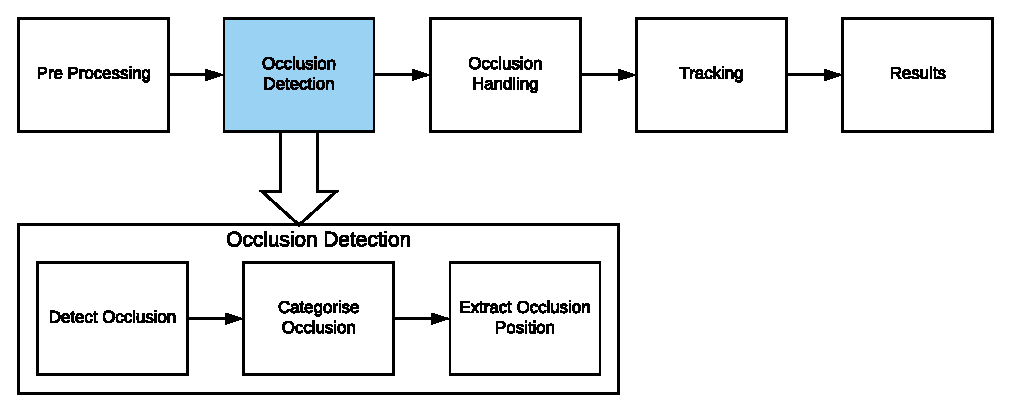
\includegraphics[width=\textwidth]{overview_flowchart}
%	\caption{Overview of an entire tracking system solution and specification of the occlusion detection part.}
%	\label{fig:overview_flow}
%\end{figure}
%
%An occlusion detection solution needs to be able to detect when and where an occlusion is occurring to be able to pass the information on to the occlusion handling process.
